%% ----------------------------------------------------------------
\section{JPEG Extractor Testing - (ms)}
%% ----------------------------------------------------------------
\label{sec:jpg_prog_test}

\subsection{Introduction}

Before the JPEG extractor can be integrated into the
AVR microcontroller, it is necessary to make sure that it is
successful in extracting the header information. This is 
achieved by coding the JPEG extractor as a C executable
file which takes in a JPEG image file and prints out the
information that it will send to the ground station software.

In order to ensure the validity of the information that is 
extracted from the JPEG file, the extractor's output is 
compared against the output of the JPEGsnoop file extractor. 
JPEGsnoop is a free Windows application which takes a 
JPEG image and outputs the information content of all 
of the JPEG file's segments \cite{hass_impulse_jpeg} .
This software provides a much more 
complete JPEG segment  information extraction and 
includes all the information extracted from the 
created JPEG extractor C executable. This is a sample
output of the JPEGSnoop application applied to the
Leaves2.jpg test image.

\begin{figure}[!hbtp]
\begin{center}
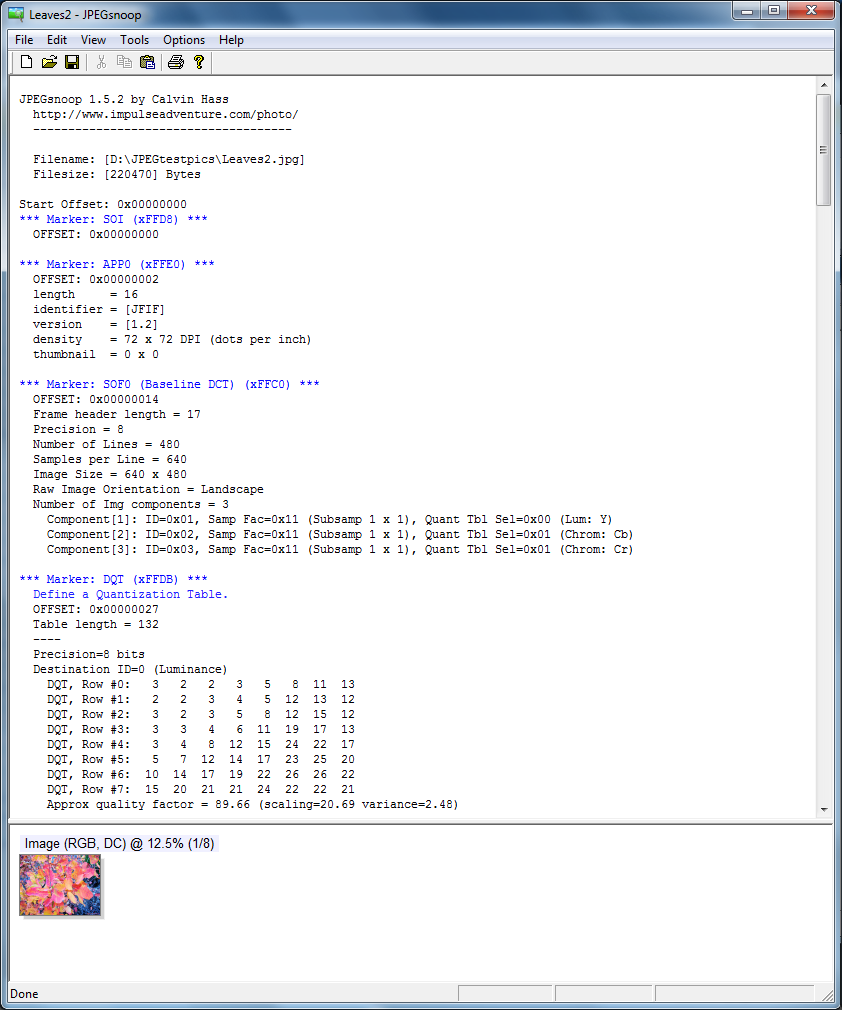
\includegraphics[scale=0.6]{figures/jpegSnoopEx1.png} 
\end{center}
\caption{JPEG segment information obtained from JPEGSnoop.exe}
\end{figure}

\newpage

The images used for the basis of the following tests
were 8 JPEG images of size 640x480 or
less. The pictures are deliberately chosen to be 
complex in order to ensure that the JPEG extractor 
can handle any image given to it by the camera.
The comparison figures below show some of the 
different images used for testing. During all 8 tests,
the output of the C executable was compared with
the output of JPEGSnoop.exe.

\subsection{Test Results}

This section will detail how the C executable's output 
was compared against the output of JPEGSnoop 
for each important JPEG segment. The C 
executable was compiled and run using
the Eclipse development platform and the output
was printed out on the Eclipse console display.

The following segments were tested:

\subsubsection{Test: SOF0}

The SOF0 information is displayed almost
identically between both outputs.
The C executable extractor does not derive the image size nor the
image orientation, because that information will
not be needed for a progressive display of the image.

\newpage

\begin{figure}[!hbtp]
\begin{center}
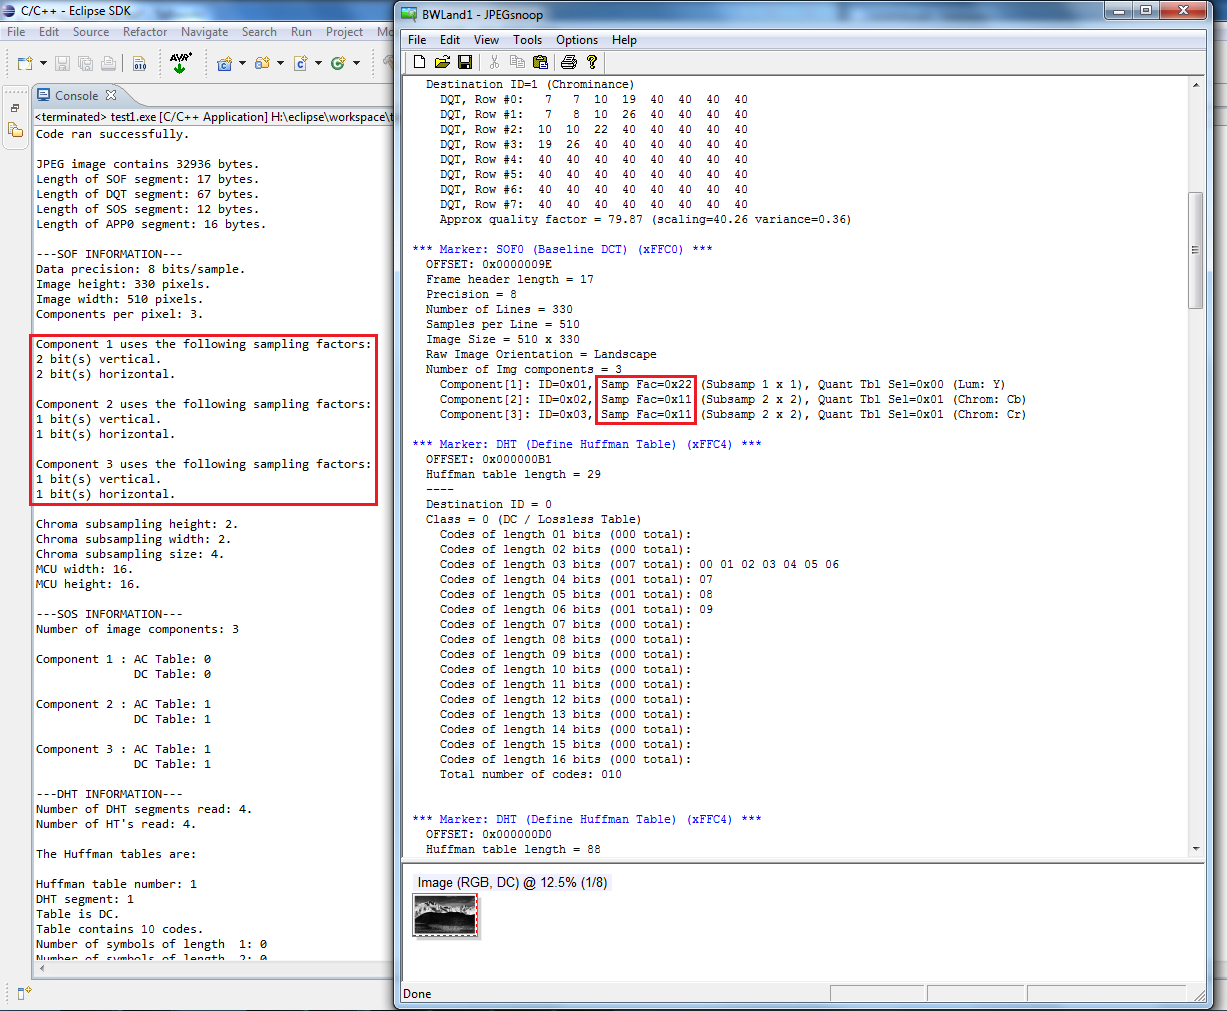
\includegraphics[scale=0.5]{figures/jpegSOFtest.png} 
\end{center}
\caption{SOF0 segment information obtained from JPEGSnoop.exe}
\end{figure}

Note that the sampling factors on each display have
been highlighted with red squares. This is to avoid 
confusion between the sampling factor and the 
subsampling factor.

\subsubsection{Test: DHT}

The extractor keeps track of the DHT segment where the Huffman
table was extracted to better understand the layout of the JPEG
file's DHT segments. The JPEGSnoop extractor simply places the
information in a more compact format compared to the display 
method used by the executable, which has no bearing on the actual
information stored.

\newpage

\begin{figure}[!hbtp]
\label{LeavesImage}
\begin{center}
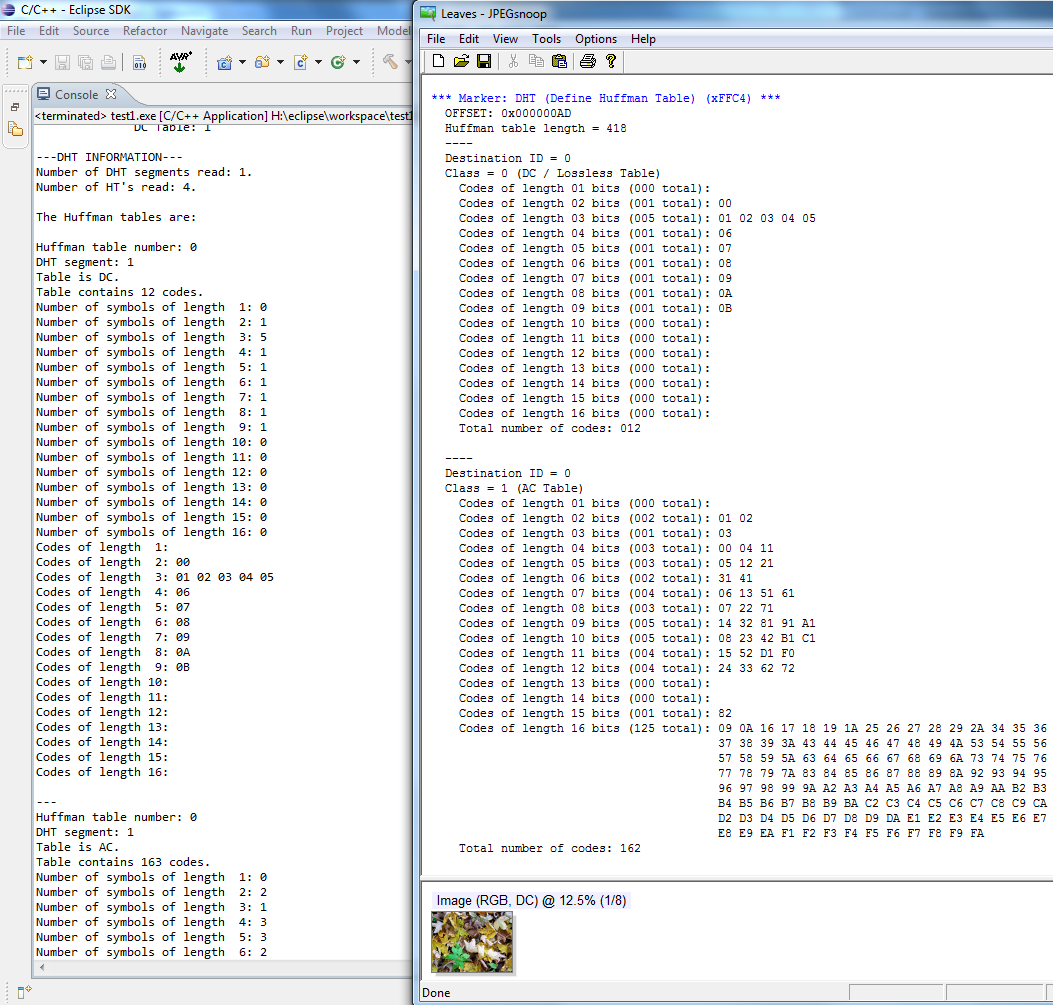
\includegraphics[scale=0.5]{figures/jpegDHTtest1.png} 
\end{center}
\caption{DHT segment information obtained from JPEGSnoop.exe}
\end{figure}

\subsubsection{Test: SOS}

The SOS segment information is read in correctly. The red squares indicate
the DHT tables which are the same in both outputs.

\newpage

\begin{figure}[!hbtp]
\begin{center}
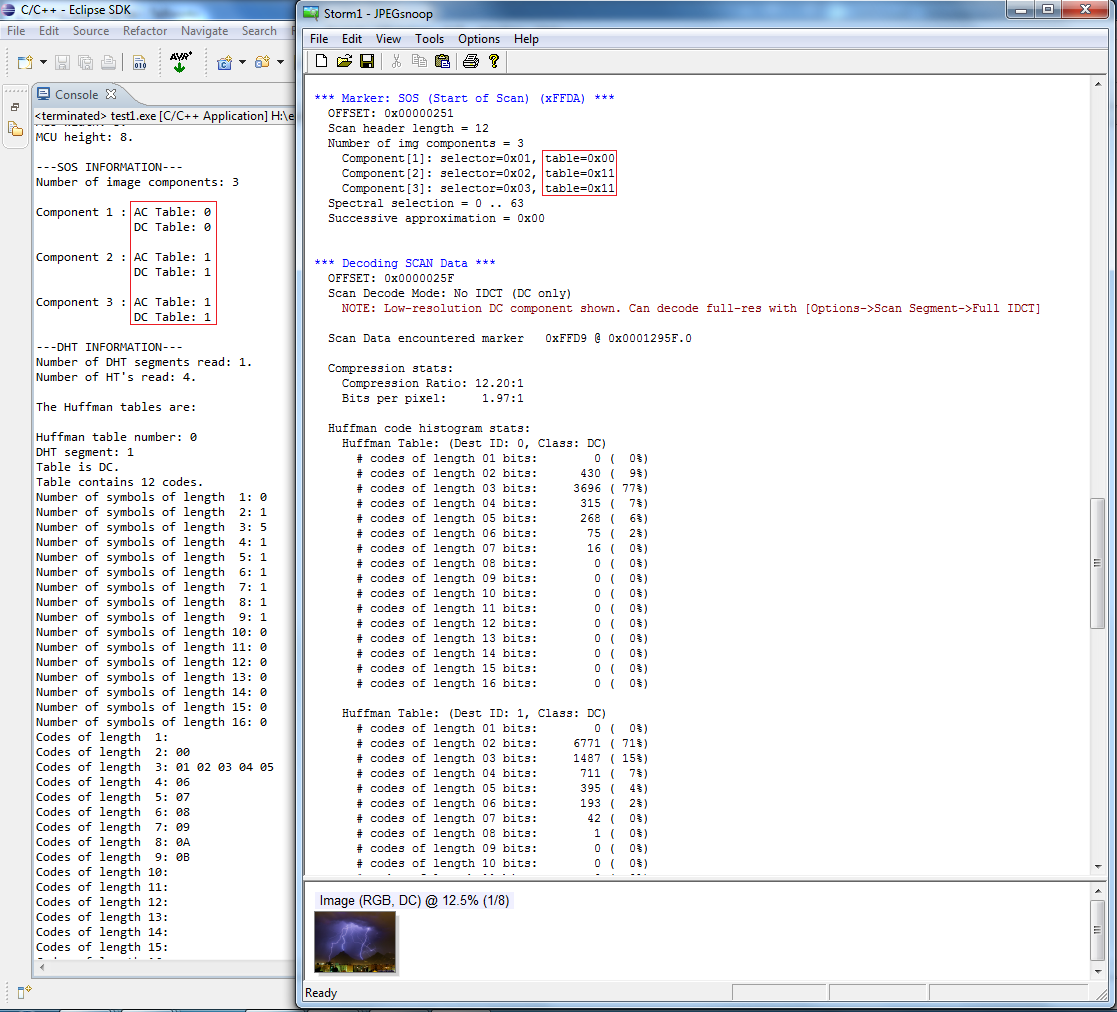
\includegraphics[scale=0.5]{figures/jpegSOStest.png} 
\end{center}
\caption{SOS segment information obtained from JPEGSnoop.exe}
\end{figure}
